
All build processes work the same way. We start from the top-level listfile and navigate downward into the project source tree. Figure 12.4 shows which project files partake in building. Numbers in parentheses indicate the order of the CMake script execution:

\begin{center}
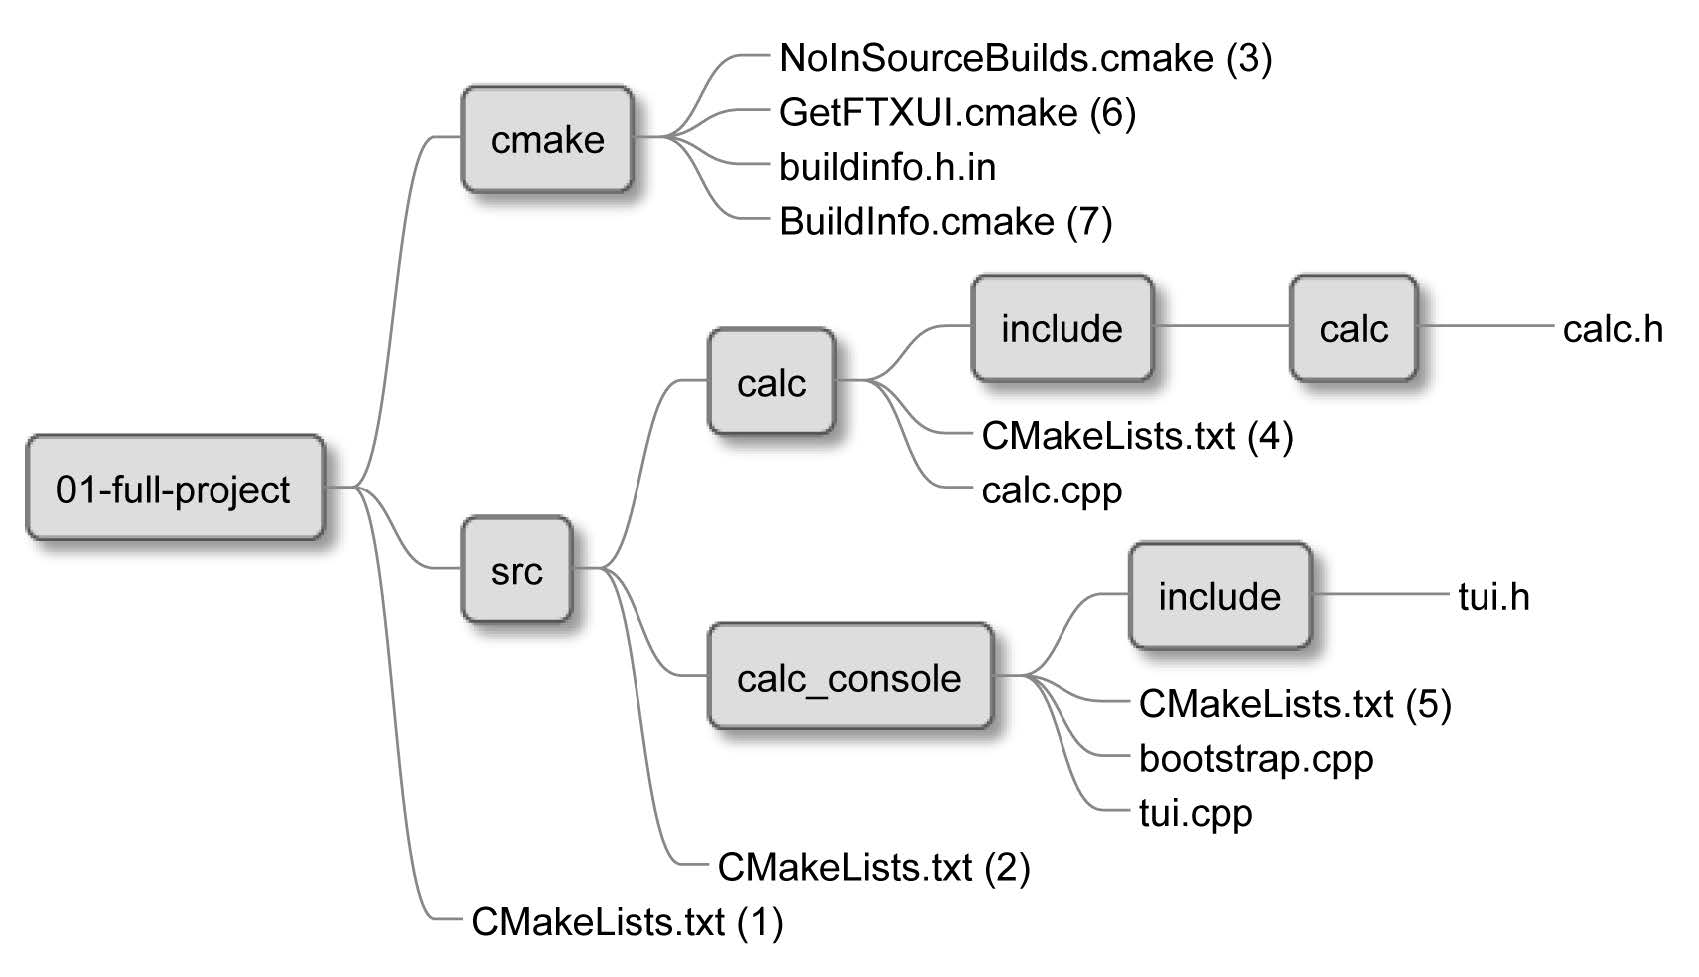
\includegraphics[width=0.8\textwidth]{content/3/chapter12/images/4.jpg}\\
Figure 12.4 – Files used in the build stage
\end{center}

Our top-level listfile will configure the project and load nested elements:

\begin{lstlisting}[style=styleCMake]
# chapter-12/01-full-project/CMakeLists.txt

cmake_minimum_required(VERSION 3.20.0)
project(Calc VERSION 1.0.0 LANGUAGES CXX)
list(APPEND CMAKE_MODULE_PATH "${CMAKE_SOURCE_DIR}/cmake")

include(NoInSourceBuilds)

add_subdirectory(src bin)
add_subdirectory(test)

include(Install)
\end{lstlisting}

We start by providing key project details and adding a path to the CMake utility modules (the cmake directory in our project). We then disable in-source builds (through a custom module) and include two key directories:

\begin{itemize}
\item 
src, containing the project source (to be named bin in the build tree)

\item 
test, containing all the testing utilities
\end{itemize}

Finally, we include another module that will set up the installation of the project. This will be discussed in another section. Meanwhile, let's take a look at the NoInSourceBuilds module to understand how it works:

\begin{lstlisting}[style=styleCMake]
# chapter-12/01-full-project/cmake/NoInSourceBuilds.cmake

if(PROJECT_SOURCE_DIR STREQUAL PROJECT_BINARY_DIR)
	message(FATAL_ERROR
		"\n"
		"In-source builds are not allowed.\n"
		"Instead, provide a path to build tree like so:\n"
		"cmake -B <destination>\n"
		"\n"
		"To remove files you accidentally created execute:\n"
		"rm -rf CMakeFiles CMakeCache.txt\n"
	)
endif()
\end{lstlisting}

No surprises here – we simply check whether the user provided a destination directory as an argument to the cmake command to store generated files. It has to be a different path than the project source tree. If that's not the case, we inform the user how to provide it and how to clean the repository after the mistake.

Our top-level listfile then includes the src subdirectory, instructing CMake to read the listfile in it:

\begin{lstlisting}[style=styleCMake]
# chapter-12/01-full-project/src/CMakeLists.txt

add_subdirectory(calc)
add_subdirectory(calc_console)
\end{lstlisting}

This file is very subtle – it simply steps into the nested directories, executing the listfiles in them. Let's follow the listfile of the calc library – it's a bit involved, so we'll discuss it in parts.

\subsubsubsection{12.4.1\hspace{0.2cm}Building the Calc library}

The list file for calc contains bits of testing configuration, but we'll focus on the building for now; the remainder will be discussed in the Testing and program analysis section:

\begin{lstlisting}[style=styleCMake]
# chapter-12/01-full-project/src/calc/CMakeLists.txt (fragment)

add_library(calc_obj OBJECT calc.cpp)
target_include_directories(calc_obj INTERFACE
	"$<BUILD_INTERFACE:${CMAKE_CURRENT_SOURCE_DIR}/include>"
	"$<INSTALL_INTERFACE:${CMAKE_INSTALL_INCLUDEDIR}>"
)
set_target_properties(calc_obj PROPERTIES
	PUBLIC_HEADER src/calc/include/calc/calc.h
	POSITION_INDEPENDENT_CODE 1
)
add_library(calc_shared SHARED)
target_link_libraries(calc_shared calc_obj)
add_library(calc_static STATIC)
target_link_libraries(calc_static calc_obj)

# ... testing and program analysis modules
# ... documentation generation
\end{lstlisting}

We declare three targets:

\begin{itemize}
\item 
calc\_obj, an object library compiling a calc.cpp implementation file. It also references the calc.h header file through the PUBLIC\_HEADER property, which can be found in the configured include directory (thanks to generator expressions providing appropriate paths for a specific mode – build or install). By using this library, we avoid repeated compilation of other targets, but we also need to enable POSITION\_INDEPENDENT\_CODE so that generated object files are usable by the shared library.

\item 
calc\_shared, a shared library depending on calc\_obj.

\item 
calc\_static, a static library depending on calc\_obj.
\end{itemize}

For completeness, we'll add a listing of the calc library's C++ code:

\begin{lstlisting}[style=styleCXX]
// chapter-12/01-full-project/src/calc/include/calc/calc.h

#pragma once

namespace Calc {
	int Sum(int a, int b);
	int Multiply(int a, int b);
} // namespace Calc
\end{lstlisting}

This code is quite basic: it declares two global functions enclosed in a Calc namespace (C++ namespaces are extremely useful in libraries, helping to avoid name collisions).

The implementation file is also very straightforward:

\begin{lstlisting}[style=styleCXX]
// chapter-12/01-full-project/src/calc/calc.cpp

namespace Calc {
int Sum(int a, int b) {
	return a + b;
}

int Multiply(int a, int b) {
	return a * b;
}
} // namespace Calc
\end{lstlisting}

This wraps up the explanation of files in the src/calc directory. Next up is the src/calc\_console and building the executable of the console calculator using this library.

\subsubsubsection{12.4.2\hspace{0.2cm}Building the Calc Console executable}

The source directory of calc\_console contains several files: a listfile, two implementation files (business code and a bootstrap), and a header file. The listfile looks as follows:

\begin{lstlisting}[style=styleCMake]
chapter-12/01-full-project/src/calc_console/CMakeLists.txt (fragment)
include(GetFTXUI)
add_library(calc_console_static STATIC tui.cpp)
target_include_directories(calc_console_static PUBLIC
	include)
target_precompile_headers(calc_console_static PUBLIC
	<string>)
target_link_libraries(calc_console_static PUBLIC
	calc_shared
	ftxui::screen ftxui::dom ftxui::component)
include(BuildInfo)
BuildInfo(calc_console_static)
# … testing and program analysis modules
# ... documentation generation

add_executable(calc_console bootstrap.cpp)
target_link_libraries(calc_console calc_console_static)
\end{lstlisting}

The listfile seem very busy, but now, as experienced CMake users, we can easily untangle what's happening inside:

\begin{itemize}
\item 
Include CMake module to fetch FTXUI dependency

\item 
Declare the calc\_console\_static target, which contains the business code, but not the main() function, to allow GTest to define its own entry point.

\item 
Add a header precompilation – we're just adding a standard string header to prove a point, but for larger projects, we could add many more (including headers belonging to the project).

\item 
Link the business code with the shared calc\_shared library and the FTXUI library.

\item 
Add all the actions to be taken on this target: the generation of build information, testing, program analysis, and documentation.

\item 
Add and link the calc\_console bootstrap executable, which provides the entry point.
\end{itemize}

Again, we'll defer discussing testing and documentation to appropriate sections in this chapter. Let's take a look at dependency management and build info generation instead.

Note that we're preferring the utility module over find-module to bring in the FTXUI. This is because it isn't very likely that this dependency is already present in the system. Rather than hoping to find it, we'll fetch and install it:

\begin{lstlisting}[style=styleCMake]
# chapter-12/01-full-project/cmake/GetFTXUI.cmake

include(FetchContent)
FetchContent_Declare(
	FTXTUI
	GIT_REPOSITORY https://github.com/ArthurSonzogni/FTXUI.git
	GIT_TAG v0.11
)
option(FTXUI_ENABLE_INSTALL "" OFF)
option(FTXUI_BUILD_EXAMPLES "" OFF)
option(FTXUI_BUILD_DOCS "" OFF)
FetchContent_MakeAvailable(FTXTUI)
\end{lstlisting}

We're using the recommended FetchContent method, described in detail in Chapter 7, Managing Dependencies with CMake. The only unusual addition is the calls of the option() command. They allow us to skip lengthy steps of the FTXUI build and disengage its installation configuration from the installation of this project. The same will be necessary for GTest dependency. The option() command is referenced in the Further reading section.

The listfile for calc\_command includes one more custom utility module that is build-related: BuildInfo. We'll use it to record three values that can be surfaced in the executable:

\begin{itemize}
\item 
SHA of the current Git commit

\item 
The timestamp of the build

\item 
The project version specified in the top-level listfile
\end{itemize}

You might remember from Chapter 5, Compiling C++ Sources with CMake, that we can use CMake to capture some build-time values and provide them to C++ code through template files – for example, with a handy C++ struct:

\begin{lstlisting}[style=styleCXX]
// chapter-12/01-full-project/cmake/buildinfo.h.in

struct BuildInfo {
	static inline const std::string CommitSHA =
		"@COMMIT_SHA@";
	static inline const std::string Timestamp =
		"@TIMESTAMP@";
	static inline const
	std::string Version = "@PROJECT_VERSION@";
};
\end{lstlisting}

To fill that structure during the configuration stage, we'll use the following code:

\begin{lstlisting}[style=styleCMake]
# chapter-12/01-full-project/cmake/BuildInfo.cmake

set(BUILDINFO_TEMPLATE_DIR ${CMAKE_CURRENT_LIST_DIR})
set(DESTINATION "${CMAKE_CURRENT_BINARY_DIR}/buildinfo")

string(TIMESTAMP TIMESTAMP)
find_program(GIT_PATH git REQUIRED)
execute_process(COMMAND
	${GIT_PATH} log --pretty=format:'%h' -n 1
	OUTPUT_VARIABLE COMMIT_SHA)

configure_file(
	"${BUILDINFO_TEMPLATE_DIR}/buildinfo.h.in"
	"${DESTINATION}/buildinfo.h" @ONLY
)

function(BuildInfo target)
	target_include_directories(${target} PRIVATE
		${DESTINATION})
endfunction()
\end{lstlisting}

Including the module will set variables containing information we're after and then we'll call configure\_file() to generate buildinfo.h. All that's left is to call the BuildInfo function and add the directory of the produced file to include directories of the desired target. The file can be then shared with multiple different consumers if needed. In such a case, you'll probably want to add include\_guard(GLOBAL) at the top of the listfile to avoid running the git command for every target.

Before delving into the implementation of the console calculator, I'd like to underline that you shouldn't worry too much about the complexity of the tui.cpp file. To fully understand it, you'll require some knowledge of the FXTUI library – we don't want to get in too deep here. Instead, let's focus on the highlighted lines:

\begin{lstlisting}[style=styleCXX]
// chapter-12/01-full-project/src/calc_console/tui.cpp

#include "tui.h"
#include <ftxui/dom/elements.hpp>
#include "buildinfo.h"
#include "calc/calc.h"

using namespace ftxui;
using namespace std;

string a{"12"}, b{"90"};
auto input_a = Input(&a, "");
auto input_b = Input(&b, "");
auto component = Container::Vertical({input_a, input_b});

Component getTui() {
	return Renderer(component, [&] {
		auto sum = Calc::Sum(stoi(a), stoi(b));
		return vbox({
			text("CalcConsole " + BuildInfo::Version),
			text("Built: " + BuildInfo::Timestamp),
			text("SHA: " + BuildInfo::CommitSHA),
			separator(),
			input_a->Render(),
			input_b->Render(),
			separator(),
			text("Sum: " + to_string(sum)),
			}) |
		border;
	});
}
\end{lstlisting}

This piece of code provides a getTui() function, which returns a ftxui::Component, an object that encapsulates an interactive UI element with labels, text fields, separators, and a border. If you're interested in how it works in detail, you'll find suitable references in the Further reading section.

More importantly, look at the include directives: they refer to the headers we provided earlier with the calc\_obj target and the BuildInfo module. The first line of the lambda function provided to the constructor of the Renderer class will call the library's Calc::Sum method and use the resulting value to print a label with sum (by calling the text() function below).

Similarly, the labels are used to present the user with the BuildInfo:: values collected at build time in three consecutive calls to text().

This method has its declaration in the related header file:

\begin{lstlisting}[style=styleCXX]
// chapter-12/01-full-project/src/calc_console/include/tui.h

#include <ftxui/component/component.hpp>
ftxui::Component getTui();
\end{lstlisting}

This is then used by the bootstrap from the calc\_console target:

\begin{lstlisting}[style=styleCXX]
// chapter-12/01-full-project/src/calc_console/bootstrap.cpp

#include <ftxui/component/screen_interactive.hpp>
#include "tui.h"

int main(int argc, char** argv) {
	ftxui::ScreenInteractive::FitComponent().Loop(getTui());
}
\end{lstlisting}

This short piece of code utilizes ftxui to create an interactive console screen that takes the Component object returned by getTui(), makes it visible to the user, and collects keyboard events in a loop, creating an interface, as shown in Figure 12.1. Again, understanding this in full isn't really crucial, as the main purpose of ftxui is to provide us with an external dependency that we can use to practice CMake techniques.

We've covered all the files in the src directory. Let's move on to the aforementioned topic of testing and analyzing the program.





